\chapter{Fine-mapping Genome-wide Association Study Summary Statistics Using Functional Annotations}

\section{Introduction}\label{sec:org59556ac}

For any particular trait, sequence-level variation at the vast majority of genetic loci is of infinitesimal consequence to that trait.  The causal
effect that a variant has on a trait induces a statistical association bewteen the presence of the variant and the trait of interest.
For a variant to have a causal effect on an organism-level trait, there must be a chain of causal events starting with the DNA-sequence,
level change, proceeding through one (or more often many) molecular intermediates, before it is observable at the organismal level.
The goal of a genome-wide association study (GWAS) is to identify a subset of variants with high statistical association with a trait of interest,
with the implicit assumption that the high degree of statistical association is the consquence of a causal relationship.
One of the major obstacles in any GWAS (or any association based statistical inference) is that the causality is but one of the means by which
a genotype may be associated with a phenotype.



Natural questions one might want to ask of this data include: what differences in gene expression between individuals who had term labors as opposed to preterm labors do we observe after accounting for other known sources of variation?;
What genes are differentially expressed between \texttt{ctr} and \texttt{dec} treated cell lines?; What genes are differentially expressed between \texttt{dec} and \texttt{TCM} cell lines?
How does the \textbf{response to treatment} (\texttt{ctr} vs \texttt{dec} and \texttt{dec} vs \texttt{TCM}) \textbf{differ} between individuals who had \textbf{term labors} and individuals who had \textbf{preterm labors}?

The key question we are asking in this project is to what extent does the genetic signal for gestational duration overlap with the observed molecular differences between placentas gathered from women who gave birth at term and preterm.

\subsection{Much of GWAS signal is non-coding}\label{sec:org3ac0b01}

Surveys of GWAS association have found that a majority of GWAS signal comes from non-coding regions of the genome.  It is believed that the majority 
of this functional variation is regulatory in nature.  Rather than modifying the function of a gene product directly, the activity of the product is modified
by modulating the abundance of the product through regulatory mechanisms: increasing or decreasing the baseline rate of transcription of DNA to RNA or degradation of mRNA back into individual nucleotides.  


\section{Materials and Methods}\label{sec:org39326e2}

\subsection{Functional Genomic Data}\label{sec:org702e301}
  
Placentas were collected from six African American women (\(\geq 18\) years old) following spontaneous labor.
Three of the women delivered at term (\(\geq 37\) weeks), and three delievered preterm.
All were vaginal deliveries of singleton pregnancies. Within 1 hour of delivery, $5 \times 5$ cm pieces of the membranes were
sampled from a distant location of the rupture site. Pieces were placed in DMEM-HAMS F12 media containing 10\% FBS and
1\% pen/strep. Samples were kept at 4°C and processed within 24 hours of tissue collection.

Primary MSC were derived from three women who delivered at term and three who delivered preterm using cells isolated from the decidua parietalis.
To model the process of decidualization, cells were treated with medroxyprogesterone acetate (MPA)
and cAMP for 48 hours and a paired set of untreated samples was cultured in parallel for 48 hours.
To model the trophoblast invasion process, cells were treated with Trophoblast Conditioned Medium (TCM).

Three replicates of of each cell line were studied to assess experimental variability in the three conditions.
Each of the 27 samples (3 individual lines x 3 replicates x 3 conditions) were assayed to generate transcriptomes (RNA-seq).
Open chromatin (ATAC-seq) was assayed for the decidualized cells and the TCM treated samples,
and histone modification (ChIP-seq) maps for H3K27ac, H3K4me1 and H3K4me3 marks were assayed in the control and decidualized cells.
Chromatin interaction was measured using promoter capture Hi-C in cultured primary decidua-derived mesenchymal stromal/stem cells (MSCs)
and in vitro differentiated decidual stromal cells (DSCs) as well as in TCM treated cells.

\subsection{Methods}\label{sec:org53944c4}


\subsubsection{Modeling Gene Expression Data}\label{sec:orgc908098}



The following sources of variation in expression data were known in addition to the primary and interaction effects: the passage number of the cell line when RNA was gathered,
the within-individual effect on gene expression, and the growth rate of the cell line.  We chose to account for the individual-level effect rather than the growth rate effect, and hoped that the estimate of the individual level effect accounts for the differences in growth rate. 

With the exception of passage number, all of the covariates of the model are categorical. There are several ways of encoding categorical variables in a generalized linear model, and different encodings can change how the coefficient
estimates are interpreted. We here briefly describe the coding of our model, with particular emphasis on the consequence of coding on the interpretation of the coefficients.  For testing which genes are differentially expressed
between control-media treated and decidualizing-media treated cells, and similarly for testing what genes are differentially expressed between decidualizing-media treated cells and trophoblast-conditioned media cells, a standard
``treatment'' coding was used wherein decidualizing-media (\texttt{dec}) was the reference level.
One can interepret the estimates for the \texttt{ctr} and \texttt{TCM} coefficients as the change in average expression in each of those condtions relative to the \texttt{dec} condition.
The effect of term vs preterm effects were estimated using a ``sum'' coding. Instead of setting either term or preterm to be a reference level, which would carry on in our interpretation of other coefficients (i.e the \texttt{ctr} and \texttt{TCM} effects would also be interpreted as relative to either \texttt{dec}-term or \texttt{dec}-preterm), the term-preterm coefficient can be interpreted as differences in the mean expression relative to one-another.
The choice of sum coding for the term vs preterm covariate is especilly important when considering how response to treatment differs between term and preterm individuals.
To formally test this hypothesis (that individuals with term births respond differently to either \texttt{dec} or \texttt{TCM} as compared to individuals with preterm births), we test for an interaction between the preterm effect
and each of the two treatment effects.  A nonzero estimate of either of these interaction terms indicates that the reponse to treatment (i.e the change in gene expression) differs between term and preterm samples.
To capture the individual level effects, instead of comparing to a particular individual, we again used a sum coding, meaning for each term and preterm,  1 covariate captures the difference between the individual 1 and individual three,and another captures the difference betweeen individual 2 and individual three.
Like passage number, individual-level effects are important to incorporate in the model, but effect-size estimates are not of direct relevance.

We used the the pseudo-alignment tool \texttt{salmon}\cite{salmon} to obtain transcript-level abundance estimates (using gencode 19 as a source of transcripts). The abundance estimates were loaded into R 
using the \texttt{tximeta} package,\cite{tximeta} which was also used to summarize the transcript-level abundance estimates into gene-level abundance estimates.  Genes with counts lower than 10 were excluded from consideration
for differential expression, as were genes for which the gene level abundance estimate was above zero in less than 5 samples.  We then used the R package \texttt{DESeq2}\cite{DESeq2} to identifiy differentially expressed genes.  For the main effect tests (i.e term vs preterm, control vs decidualized, and TCM vs decidualized)  we used the Wald test functionality for null hypothesis significance testing.  \texttt{DESeq2} includes composite null hypothesis testing functionality when using the Wald test; instead of testing against the null hypothesis  that \(\beta =  0\), one can test against the hypothesis that \(\lvert \beta \rvert \leq \theta\) where \(\theta\) is some threshold value.  Rather than adding a fold-change cutoff on top of a test against an effect size of 0,  with the composite test the FDR results remain interpretable: \$p\$-values and adjusted \$p\$-values correspond to the specific null hypothesis of interest.  This composite null-hypothesis testing was used with a log fold-change threshold of 0.2.

\subsubsection{A pipeline for fine-mapping GWAS summary statistics using functional annotations}\label{sec:org24e3fbe}

Fine mapping proceeded in three stages. In the first stage we partitioned the genome into 1,703 regions approximately independent regions using breakpoints derived from the ldetect method\cite{ldetect}.
Next, we constructed a SNP-level prior probability of causality, informed by the functional genomic datathat a particular SNP is causal.  To estimate the functionally informed SNP-level prior, We employed a Bayesian
hierarchical model TORUS\cite{torus}.  TORUS uses SNP-level annotations and GWAS summary statistics to estimate the extent to which SNPs with functional genomic annotations are likely to be causal for a trait of interest.  
TORUS takes as input GWAS summary statistics and genomic annotations, and for each annotation outputs multivariate enrichment estimates that corresponding to estimates from a logistic regression: 
the additive change in log odds for a variant being causal, conditioned on all other annotations being held constant.We ran TORUS with the gestational age GWAS summary statistics and the reproducible
H3K27ac and H3K4me1 peaks from the \texttt{dec}-treated samples, the pcHi-C contact regions, and the union of all ATAC-seq peaks to obtain enrichment estimates. A SNP-level prior was constructed from those enrichment estimates.
Lastly, fine mapping was performed using a summary statistics-based version of the “Sum of Single Effects” model (SuSiE\cite{susie}).  
In the summary statistics-based version of SuSiE, the inputs are the GWAS summary statistics in a region, the SNP-level prior for every GWAS variant, and an estimate of the LD between variants. 
As an estimate of LD, we used the unrelated European individuals from the 1000 Genomes project as a reference panel. SuSiE (as implemented in the R package “susieR”) was run on the 33 regions most 
believed to have one or more causal variants as estimated by TORUS. For each region, SuSiE was run with a uniform prior (default setting of SuSiE) and with an informed prior learned 
by TORUS. The parameter $L$ of SuSiE (maximum number of causal variants) is set at 3 when running SuSiE.  To be conservative, the pip for all SNPs in each region were multiplied by $1-\text{FDR}_{\text{TORUS}}$ to approximate the
TORUS posterior probability that the region contained at least one causal variant.

% This conservative setting ensures that the results are robust to possible LD mismatch between 
% the reference panel and the GWAS samples. In fact, when $L = 1$, the PIP of a SNP depends only on its summary statistic (effect size and standard error), prior effect size and the number of SNPs in the locus, 
% but not LD structure.  


% \subsubsection{Stratified LD score regression}\label{sec:org3173e32}

% We assessed how much of the heritability of  gestational duration is contained within ATAC-seq, H3K4me1, H3K4me3, H3K27ac and pcHi-C peaks using stratified LD score regression (S-LDSC).
% Stratified LD score regression is a generalization of LD score regression, a method for estimating the heritability of a trait using SNP-level GWAS summary statistics and SNP-level estimates
% of the amount of genetic variation tagged at each variant, known as LD scores.  Under the LD-score regression model, the expected value of the GWAS summary statistic for a variant
% (specifically 
% the expected value of the \(\chi^2\) statistic) is a linear function of the LD score at that site, and h2, the per-SNP heritability, and a an intercept parameter.  Under the S-LDSC
% model, rather than estimating a single per-SNP heritability parameter, a parameter is estimated for each of several functional annotations.  In a standard S-LDSC analysis,
% user-provided annotations are combined with a ``baseline'' set of genomicannotations from publicly available datasets.  For this analysis, stratified LD scores were calculated using
% the peaks identified as reproducible across either treated or untreated samples as annotations and the  1000 Genomes Phase 3 European individuals (Price Lab website) as a reference
% LD panel, using only the HapMap3 SNP list (also from the Price Lab website). Stratified LD regression was performed on the gestational duration GWAS using the endometrial-tissue
% derived LD scores and the “baseline” LD scores contained in version 2.2 of the LD score regression baseline LD model. We include all annotations from the baseline LD model 
% except those “flanking” annotations. This resulted in a total of 64 baseline annotations used in our S-LDSC analysis.  



\subsubsection{Gene-level summary of fine-mapping results}\label{sec:org3f48450}

To assess the enrichment of the gestational duration GWAS signal the differential expression gene signal we developed a method for summarizing our fine-mapping results at the gene level.  SNP-level PIPs were summarized as gene-level
PIPs based on one of several SNP to gene associations, and accounting for uncertainty in which gene the SNP targets.  SNPs in the \(5'\) UTR (or 2kb upstream of the \(5'\) UTR), \(3'\) UTR, or exon for a gene were assigned to that gene
, and the entire PIP for that variant is added to the total for that gene. A SNP that is within a promoter-capture HiC contact, (as called by CHiCAGO \cite{chicago}) is assigned the gene corresponding to the promoter of the
promoter-target pair.  The entire PIP for the variant is assigned to the total for the gene, unless the variant is in HiC contact with multiple promoters, in which case the PIP is split equally between the multiple genes.
If the target, i.e the non-promoter region in the promoter-capture HiC contact, lies within the gene body (the \(5'\) UTR, the \(3'\) UTR, or an exon) of a gene, that SNP is assigned to both the gene containing the variant
as well as the gene corresponding to the promoter of the promoter-capture HiC contact, and the PIP for that variant is split equally between the gene-level totals for both genes.
For variants that lay outside genes or HiC contacts, the a portion of the PIP for that variant was assigned to each gene within the fine-mapping region, with the proportion decaying exponentially with distance to the gene according
to the following function
$$\rho_{i,g}\frac{e^{\frac{-d_{i,g}}{100000}}}{\sum_{j=1}^G e^{\frac{-d_{i,j}}{100000}}}$$, with $d_{i,g}$ being the minimum distance between variant $i$ and any of gene $g$'s exons, \(5'\) UTR or \(3'\) UTR.  

We take the simplifying assumption that causal variants act through exactly one (annotated) gene. We use the following equation for the gene-level PIP:

$$\text{P}_{g} = \sum_{i \in H_g}  \frac{p_i}{h_i} + \sum_{j \in B_g} p_j + \sum_{k \not\in H_g \cup B_g} \rho_{k,g}p_k$$

In the above equation $H_g$ is the set of variants in HiC contact with gene $g$, $h_i$ is the number of HiC contacts in contact with variant $i$, $B_g$ is the set of variants within the \(5'\) UTR, the \(3'\) UTR, or an exon of gene $g$, and $H_g \cup B_g$ is the union of $H_g$ and $B_g$.

\section{Results}\label{sec:orgb8d6bf0}


\subsection{Enrichment for Gestational Duration GWAS signal in Decidual Derived Functional Annotations}

\begin{figure}
  \centering
  \begin{subfigure}[t]{\textwidth}
    \centering
    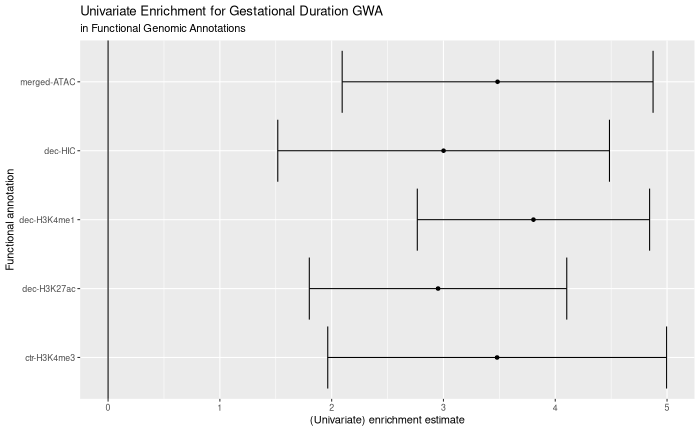
\includegraphics[width=\linewidth]{img/ptb_univ_assoc.png}
    \caption{Univariate enrichment for gestational duration GWAS signal in regulatory maps of decidua-derived stromal cells. TORUS was run on each }\label{fig:univ_assoc}
  \end{subfigure}
    \begin{subfigure}[t]{\textwidth}
    \centering
    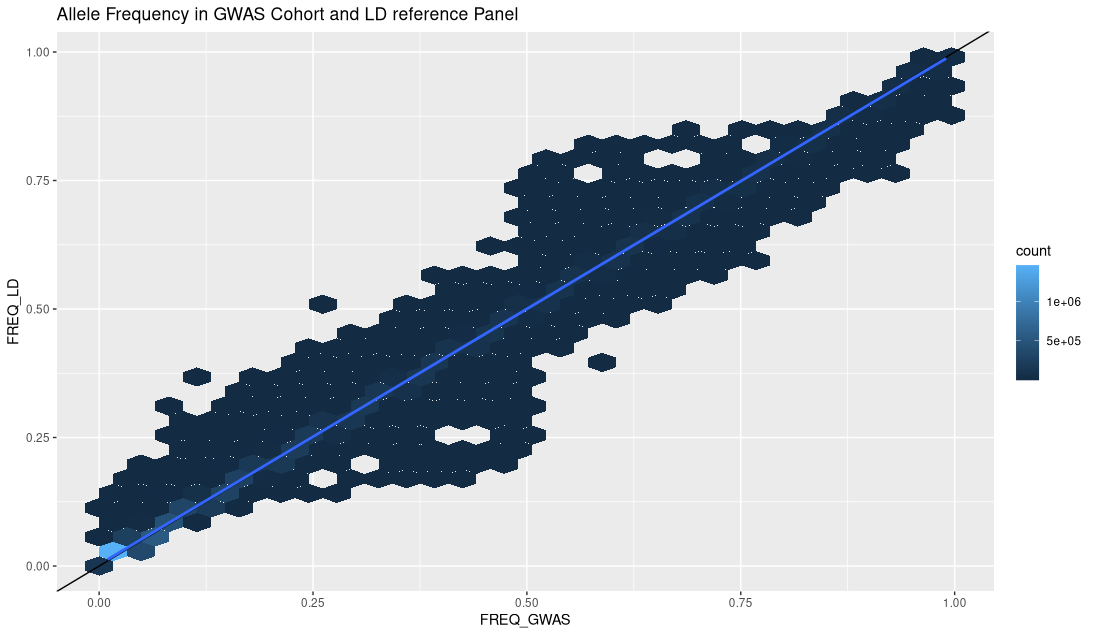
\includegraphics[width=\linewidth]{img/Allele_freq_match.png}
    \caption{}\label{fig:multiv_assoc}
    \end{subfigure}
\end{figure}



\section{Discussion}\label{sec:org53f1196}

